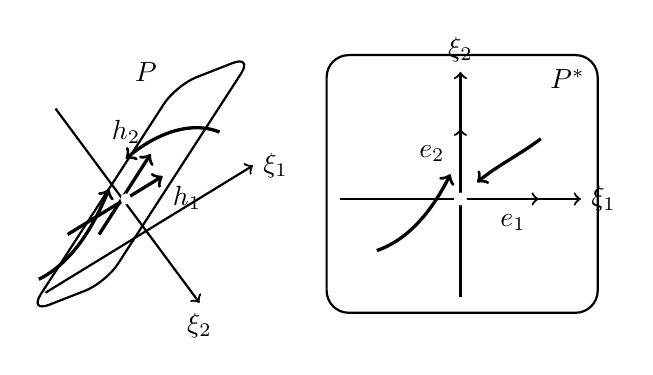
\begin{tikzpicture}[x=0.85cm,y=0.85cm,thick]
  % Oblique plane P and its eigenbasis.
  \draw[rounded corners=8pt] (-4.0,-1.65)--(-1.8,1.75)--(-0.65,2.2)--(-2.85,-1.2)--cycle;
  \coordinate (O) at (-2.55,0.05);
  \draw[->] (-3.75,-1.35)--(-0.65,0.55) node[right] {$\xi_1$};
  \draw[->] (-3.6,1.4)--(-1.45,-1.5) node[below] {$\xi_2$};
  \draw[->,very thick] (-3.42,-0.48)--(-2.0,0.39);
  \draw[->,very thick] (-2.95,-0.48)--(-2.18,0.72);
  \node[below right] at (-2.0,0.39) {$\vect{h}_1$};
  \node[above left] at (-2.18,0.72) {$\vect{h}_2$};
  \fill[white] (O) circle (2pt);
  \node at (-2.25,1.95) {$P$};
  % Sample trajectories in the skew plane.
  \draw[->,very thick] (-3.85,-1.15) .. controls (-3.25,-0.85) and (-2.95,-0.15) .. (-2.8,0.2);
  \draw[->,very thick] (-1.15,1.05) .. controls (-1.65,1.25) and (-2.2,0.95) .. (-2.55,0.65);
  % Affine image P*: orthogonal coordinate axes and corresponding trajectories.
  \draw[rounded corners=8pt] (0.45,-1.65) rectangle (4.5,2.2);
  \draw[->] (0.65,0.05)--(4.25,0.05) node[right] {$\xi_1$};
  \draw[->] (2.45,-1.42)--(2.45,1.95) node[above] {$\xi_2$};
  \draw[->,very thick] (1.2,-0.72) .. controls (1.7,-0.55) and (2.05,-0.08) .. (2.3,0.42);
  \draw[->,very thick] (3.65,0.95) .. controls (3.35,0.72) and (3.0,0.55) .. (2.7,0.3);
  \draw[->] (2.85,0.05)--(3.62,0.05) node[midway,below=2pt] {$\vect{e}_1$};
  \draw[->] (2.45,0.36)--(2.45,1.10) node[midway,left=2pt] {$\vect{e}_2$};
  \fill[white] (2.45,0.05) circle (2.3pt);
  \node at (4.05,1.85) {$P^*$};
\end{tikzpicture}
